\section{Algorithm}


\begin{algorithm}
  \caption{\hskip0.5em 2D Generalized Hilbert Function (Gilbert2D) } %($p$, $\alpha$, $\beta$) \\ \hskip3.0em $p, \alpha, \beta \in \mathbb{Z}^3$ }
  \label{alg:gilbert2d}
  \begin{algorithmic}

    \Function{Gilbert2D}{$p$, $\alpha$, $\beta$}
      \State
      \State $\alpha_2, \beta_2  = (\alpha // 2), (\beta // 2)$

      \State
      \If{ $(|\beta| \equiv 1)$ }
        \State \textbf{yield} $p + i \cdot \delta(\alpha)$ \textbf{forall} $i \in |\alpha|$

        \State
      \ElsIf{ $(|\alpha| \equiv 1)$ }
        \State \textbf{yield} $p + i \cdot \delta(\alpha)$ \textbf{forall} $i \in |\beta|$

        \State
      \ElsIf{ $(2 |\alpha| > 3 |\beta|)$ }
        \If{ $(|\alpha_2| > 2)$ and $(|\alpha_2| \bmod{2} \equiv 1)$ }
          \State $\alpha_2 \leftarrow \alpha_2 + \delta(\alpha)$
        \EndIf
        \State
        \State \textbf{yield} Gilbert2D($p$, \\ \hskip9.75em $\alpha_2$, $\beta$)
        \State
        \State \textbf{yield} Gilbert2D($p + \alpha_2$, \\ \hskip9.75em $\alpha - \alpha_2$, $\beta$)

        \State
      \Else
        \If{ $(|\beta_2| > 2)$ and $(|\beta_2| \bmod{2} \equiv 1)$ }
          \State $\beta_2 \leftarrow \beta_2 + \delta(\beta)$
        \EndIf
        \State
        \State \textbf{yield} Gilbert2D($p$, \\ \hskip9.75em $\beta_2$, $\alpha_2$)
        \State
        \State \textbf{yield} Gilbert2D($p + \beta_2$, \\ \hskip9.75em $\alpha$, $(\beta - \beta_2)$)
        \State
        \State \textbf{yield} Gilbert2D($p + \alpha - \delta(\alpha) + \beta_2 - \delta(\beta)$, \\ \hskip9.75em $\beta_2$, $-(\alpha - \alpha_2)$)
      \EndIf
    \EndFunction
  \end{algorithmic}
\end{algorithm}

\floatname{algorithm}{Procedure}

\begin{algorithm}
  \caption{ \hskip0.5em $S_0$-Split function (eccentric split) }
  \label{alg:procS0}
  \begin{algorithmic}
    \State
    \State \textit{\# split halfway on $\alpha$ }
    \Function{$S_0$}{$p$, $\alpha$, $\beta$, $\gamma$}
      \State $\alpha_2 \leftarrow (\alpha // 2)$
      \If{ $(|\alpha| > 2)$ and $((|\alpha_2| \bmod{2}) \equiv 1)$ }
        \State $\alpha_2 \leftarrow \alpha_2 + \delta(\alpha)$
      \EndIf
      \State
      \State \textbf{yield} Gilbert3D($p$, \\ \hskip8.25em $\alpha_{2}$, $\beta$, $\gamma$ )
      \State
      \State \textbf{yield} Gilbert3D($p + \alpha_{2}$, \\ \hskip8.25em $(\alpha - \alpha_{2})$, $\beta$, $\gamma$ )
    \EndFunction
  \end{algorithmic}
\end{algorithm}


\begin{algorithm}
  \caption{ \hskip0.5em $S_1$-Split functions (eccentric split) }
  \label{alg:procS1}
  \begin{algorithmic}
    \State
    \State \textit{\# split $\frac{1}{3}$ on $\gamma$ and halfway on $\alpha$ }
    \Function{$S_1$}{$p$, $\alpha$, $\beta$, $\gamma$}
      \State $\alpha_2, \gamma_3 \leftarrow (\alpha // 2), (\gamma // 3)$
      \If{ $(|\alpha| > 2)$ and $((|\alpha_2| \bmod{2}) \equiv 1)$ }
        \State $\alpha_2 \leftarrow \alpha_2 + \delta(\alpha)$
      \EndIf
      \If{ $(|\gamma| > 2)$ and $((|\gamma_3| \bmod{2}) \equiv 1)$ }
        \State $\gamma_3 \leftarrow \gamma_3 + \delta(\gamma)$
      \EndIf
      \State
      \State \textbf{yield} Gilbert3D($p$, \\ \hskip8.25em $\gamma_3$, $\alpha_2$, $\beta$)
      \State
      \State \textbf{yield} Gilbert3D($p + \gamma_3$, \\ \hskip8.25em $\alpha$, $\beta$, $(\gamma - \gamma_3)$)
      \State
      \State \textbf{yield} Gilbert3D($p + \alpha - \delta(\alpha) + \gamma_{3} - \delta(\gamma)$, \\ \hskip8.25em $\gamma_3$, $(\alpha - \alpha_2)$, $\beta$)
    \EndFunction
  \end{algorithmic}
\end{algorithm}


\begin{algorithm}
  \caption{ \hskip0.5em $S_2$-Split function (eccentric split) }
  \label{alg:procS2}
  \begin{algorithmic}
    \State
    \State \textit{\# split $\frac{1}{3}$ on $\beta$ and halfway on $\alpha$ }
    \Function{$S_2$}{$p$, $\alpha$, $\beta$, $\gamma$}
      \State $\alpha_2, \beta_3 \leftarrow (\alpha // 2), (\beta // 3)$
      \If{ $(|\alpha| > 2)$ and $((|\alpha_2| \bmod{2}) \equiv 1)$ }
        \State $\alpha_2 \leftarrow \alpha_2 + \delta(\alpha)$
      \EndIf
      \If{ $(|\beta| > 2)$ and $((|\beta_3| \bmod{2}) \equiv 1)$ }
        \State $\beta_3 \leftarrow \beta_3 + \delta(\beta)$
      \EndIf
      \State
      \State \textbf{yield} Gilbert3D($p$, \\ \hskip8.25em $\beta_{3}$, $\gamma$, $\alpha_2$ )
      \State
      \State \textbf{yield} Gilbert3D($p + \beta_{3}$, \\ \hskip8.25em $\alpha$, $(\beta - \beta_{3})$, $\gamma$ )
      \State
      \State \textbf{yield} Gilbert3D($p + \alpha - \delta(\alpha) + \beta_{3} - \delta(\beta)$, \\ \hskip8.25em $-\beta_{3}$, $\gamma$, $-\alpha$)
    \EndFunction
  \end{algorithmic}
\end{algorithm}


\begin{algorithm}
  \caption{ \hskip0.5em $J_0$-Split function }
  \label{alg:procJ0}
  \begin{algorithmic}
    \State
    \State \textit{\# $|\gamma|$ even }
    \Function{$J_0$}{$p$, $\alpha$, $\beta$, $\gamma$}
      \State
      \State $\alpha_2, \beta_2, \gamma_2 \leftarrow (\alpha // 2), (\beta // 2), (\gamma // 2)$
      \State
      \State \textit{\# prefer initial block even}
      \State $\alpha_2=\alpha_2+\delta(\alpha)$ \textbf{if} $(|\alpha_2| > 2)$and$(|\alpha_2| \bmod{2} \equiv 1)$
      \State $\beta_2=\beta_2+\delta(\beta)$ \textbf{if} $(|\beta_2| > 2)$and$(|\beta_2| \bmod{2} \equiv 1)$
      \State $\gamma_2=\gamma_2+\delta(\gamma)$ \textbf{if} $(|\gamma_2| > 2)$and$(|\gamma_2| \bmod{2} \equiv 1)$
      \State
      \State \textbf{yield} Gilbert3D($p$, \\ \hskip8.25em $\beta_2$, $\gamma_2$, $\alpha_2$)
      \State
      \State \textbf{yield} Gilbert3D($p+\beta_2$, \\ \hskip8.25em $\gamma$, $\alpha_2$, $\beta - \beta_2$)
      \State
      \State \textbf{yield} Gilbert3D($p + \beta_2 - \delta(\beta_2) + \gamma - \delta(\gamma)$, \\ \hskip8.25em $\alpha$, $-\beta_2$, $-(\gamma - \gamma_2)$)
      \State
      \State \textbf{yield} Gilbert3D($p + \alpha - \delta(\alpha) + \beta_2 + \gamma - \delta(\gamma)$, \\ \hskip8.25em $-\gamma$, $-(\alpha - \alpha_2)$, $(\beta - \beta_2)$)
      \State
      \State \textbf{yield} Gilbert3D($p + \alpha - \delta(\alpha) + \beta_2 - \delta(\beta)$, \\ \hskip8.25em $-\beta_2$, $\gamma_2$, $-(\alpha - \alpha_2)$)
    \EndFunction
  \end{algorithmic}
\end{algorithm}


\begin{algorithm}
  \caption{ \hskip0.5em $J_1$-Split function }
  \label{alg:procJ2}
  \begin{algorithmic}
    \State
    \State \textit{\# $|\gamma|$ odd, one of $|\alpha|$ or $|\beta|$ even }
    \Function{$J_1$}{$p$, $\alpha$, $\beta$, $\gamma$}
      \State
      \State $\alpha_2, \beta_2, \gamma_2 \leftarrow (\alpha // 2), (\beta // 2), (\gamma // 2)$
      \State
      \State \textit{\# prefer $\beta_2$, $\gamma_2$ even but force $\alpha_2$ odd }
      \State $\alpha_2=\alpha_2+\delta(\alpha)$ \textbf{if} $(|\alpha_2| > 2)$and$(|\alpha_2| \bmod{2} \equiv 0)$
      \State $\beta_2=\beta_2+\delta(\beta)$ \textbf{if} $(|\beta_2| > 2)$and$(|\beta_2| \bmod{2} \equiv 1)$
      \State $\gamma_2=\gamma_2+\delta(\gamma)$ \textbf{if} $(|\gamma_2| > 2)$and$(|\gamma_2| \bmod{2} \equiv 1)$
      \State
      \State \textbf{yield} Gilbert3D($p$, \\ \hskip8.25em $\gamma2$, $\alpha_2$, $\beta_2$)
      \State
      \State \textbf{yield} Gilbert3D($p+\gamma_2$, \\ \hskip8.25em $\beta$, $\gamma - \gamma_2$, $\alpha_2$)
      \State
      \State \textbf{yield} Gilbert3D($p+\gamma_2 - \delta(\gamma) + \beta - \delta(\beta)$, \\ \hskip8.25em $\alpha$, $-(\beta - \beta_2)$, $-\gamma_2$)
      \State
      \State \textbf{yield} Gilbert3D($p+\alpha - \delta(\alpha) + \beta - \delta(\beta) + \gamma_2 - \delta(\gamma)$, \\ \hskip8.25em $\beta$, $\gamma - \gamma_2$, $-(\alpha - \alpha_2)$)
      \State
      \State \textbf{yield} Gilbert3D($p+\alpha - \delta(\alpha) + \gamma_2 - \delta(\gamma)$, \\ \hskip8.25em $-\gamma_2$, $-(\alpha - \alpha_2)$, $\beta_2$)
    \EndFunction
  \end{algorithmic}
\end{algorithm}


\begin{algorithm}
  \caption{ \hskip0.5em $J_2$-Split function }
  \label{alg:procJ2}
  \begin{algorithmic}
    \State
    \State \textit{\# $|\alpha|, |\beta|, |\gamma|$ odd }
    \Function{$J_2$}{$p$, $\alpha$, $\beta$, $\gamma$}
      \State
      \State $\alpha_2, \beta_2, \gamma_2 \leftarrow (\alpha // 2), (\beta // 2), (\gamma // 2)$
      \State
      \State \textit{\# prefer $\beta_2$, $\gamma_2$ even but force $\alpha_2$ odd }
      \State $\alpha_2=\alpha_2+\delta(\alpha)$ \textbf{if} $(|\alpha_2| > 2)$and$(|\alpha_2| \bmod{2} \equiv 0)$
      \State $\beta_2=\beta_2+\delta(\beta)$ \textbf{if} $(|\beta_2| > 2)$and$(|\beta_2| \bmod{2} \equiv 1)$
      \State $\gamma_2=\gamma_2+\delta(\gamma)$ \textbf{if} $(|\gamma_2| > 2)$and$(|\gamma_2| \bmod{2} \equiv 1)$
      \State
      \State \textbf{yield} Gilbert3D($p$, \\ \hskip8.25em $\beta_2$, $\gamma$, $\alpha_2$)
      \State
      \State \textbf{yield} Gilbert3D($p+\beta_2$, \\ \hskip8.25em $\gamma_2$, $\alpha$, $(\beta - \beta_2)$)
      \State
      \State \textbf{yield} Gilbert3D($p+\beta_2 + \gamma_2$, \\ \hskip8.25em $\alpha$, $(\beta - \beta_2)$, $(\gamma - \gamma_2)$)
      \State
      \State \textbf{yield} Gilbert3D($p + \alpha - \delta(\alpha) + \beta_2 - \delta(\beta) + \gamma_2$, \\ \hskip8.25em $-\beta_2$, $(\gamma- \gamma_2)$, $-(\alpha - \delta(\alpha))$)
      \State
      \State \textbf{yield} Gilbert3D($p + \alpha - \delta(\alpha) + \gamma_2 - \delta(\gamma)$, \\ \hskip8.25em $-\gamma_2$, $-(\alpha - \alpha_2)$, $\beta_2$)
    \EndFunction
  \end{algorithmic}
\end{algorithm}

\floatname{algorithm}{Algorithm}

\begin{algorithm}
  \caption{ \hskip0.5em 3D Generalized Hilbert Function (Gilbert3D) } %($p$, $\alpha$, $\beta$, $\gamma$) \\ \hskip3.0em $p, \alpha, \beta, \gamma \in \mathbb{Z}^3$ }
  \label{alg:gilbert3d}
  \begin{algorithmic}
    \Function{Gilbert3D}{$p$, $\alpha$, $\beta$, $\gamma$}

    \State
    \State\textit{\# Parity of dimensions}

    \State $\alpha_0 \leftarrow (|\alpha|\bmod{2})$
    \State $\beta_0 \leftarrow (|\beta|\bmod{2})$
    \State $\gamma_0 \leftarrow (|\gamma|\bmod{2})$

    \State
    \State\textit{\# Base cases }
    \State \textbf{if} ($(|\alpha|\equiv 2)$ and $(|\beta|\equiv 2)$ and $(|\gamma| \equiv 2)$)
    \State \hskip1.5em \Return Hilbert3D($p$,$\alpha$,$\beta$,$\gamma$) 
    \State \Return Gilbert2D($p$,$\beta$,$\gamma$) \textbf{if} $(|\alpha| \equiv 1)$
    \State \Return Gilbert2D($p$,$\alpha$,$\gamma$) \textbf{if} $(|\beta| \equiv 1)$
    \State \Return Gilbert2D($p$,$\alpha$,$\beta$) \textbf{if} $(|\gamma| \equiv 1)$

    \State
    \State\textit{\# Eccentric cases }

    \State \textbf{if }$(3 |\alpha|>5|\beta|) \text{ and } (3|\alpha|>5|\gamma|))$
    \State \hskip1.5em \Return $S _ 0$($p$,$\alpha$,$\beta$,$\gamma$) 
    \State \textbf{if }$(2 |\beta| > 3 |\gamma|) \text{ or }(2 |\beta| > 3 |\alpha|))$
    \State \hskip1.5em \Return $S _ 2$($p$,$\alpha$,$\beta$,$\gamma$)
    \State \textbf{if }$(2 |\gamma| > 3 |\beta|)$
    \State \hskip1.5em \Return $S _ 1$($p$,$\alpha$,$\beta$,$\gamma$)

    \State
    \State \textit{\# Bulk recursion }
    \State \Return $J _ 0$($p$,$\alpha$,$\beta$,$\gamma$) \textbf{if} $(\gamma_0 \equiv 0)$
    \State \Return $J _ 1$($p$,$\alpha$,$\beta$,$\gamma$) \textbf{if} $(\alpha_0 \equiv 0)$or$(\beta_0\equiv 0)$
    \State \Return $J _ 2$($p$,$\alpha$,$\beta$,$\gamma$)

    \EndFunction

  \end{algorithmic}
\end{algorithm}

\begin{figure}[h]
  \centering
  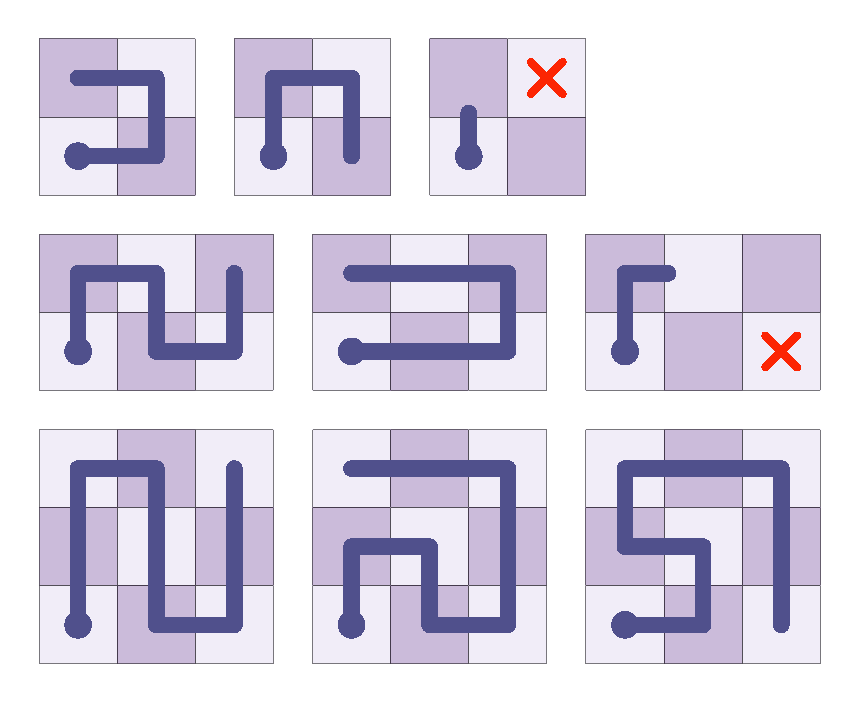
\includegraphics[width=\linewidth]{simple_hampath.pdf}
  \caption{ Illustrative examples of Hamiltonian paths height/width that are even/even, even/odd and odd/odd, respectively,
            when starting from the lower left hand corner }
  \label{fig:exampleHampath}
\end{figure}


\begin{figure}[h]
  \centering
  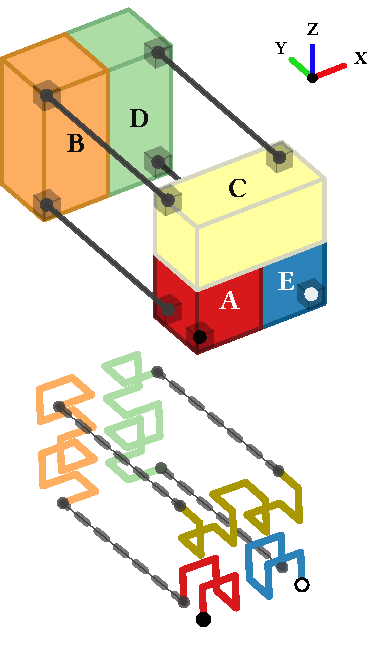
\includegraphics[width=\linewidth]{gilbert3d_explode.pdf}
  \caption{ The J-split subdivision, representing the main subdivision of the build recursion for the 3D Gilbert curve case }
  \label{fig:gilbert3DJSplit}
\end{figure}


\begin{figure*}[ht]
  \centering
  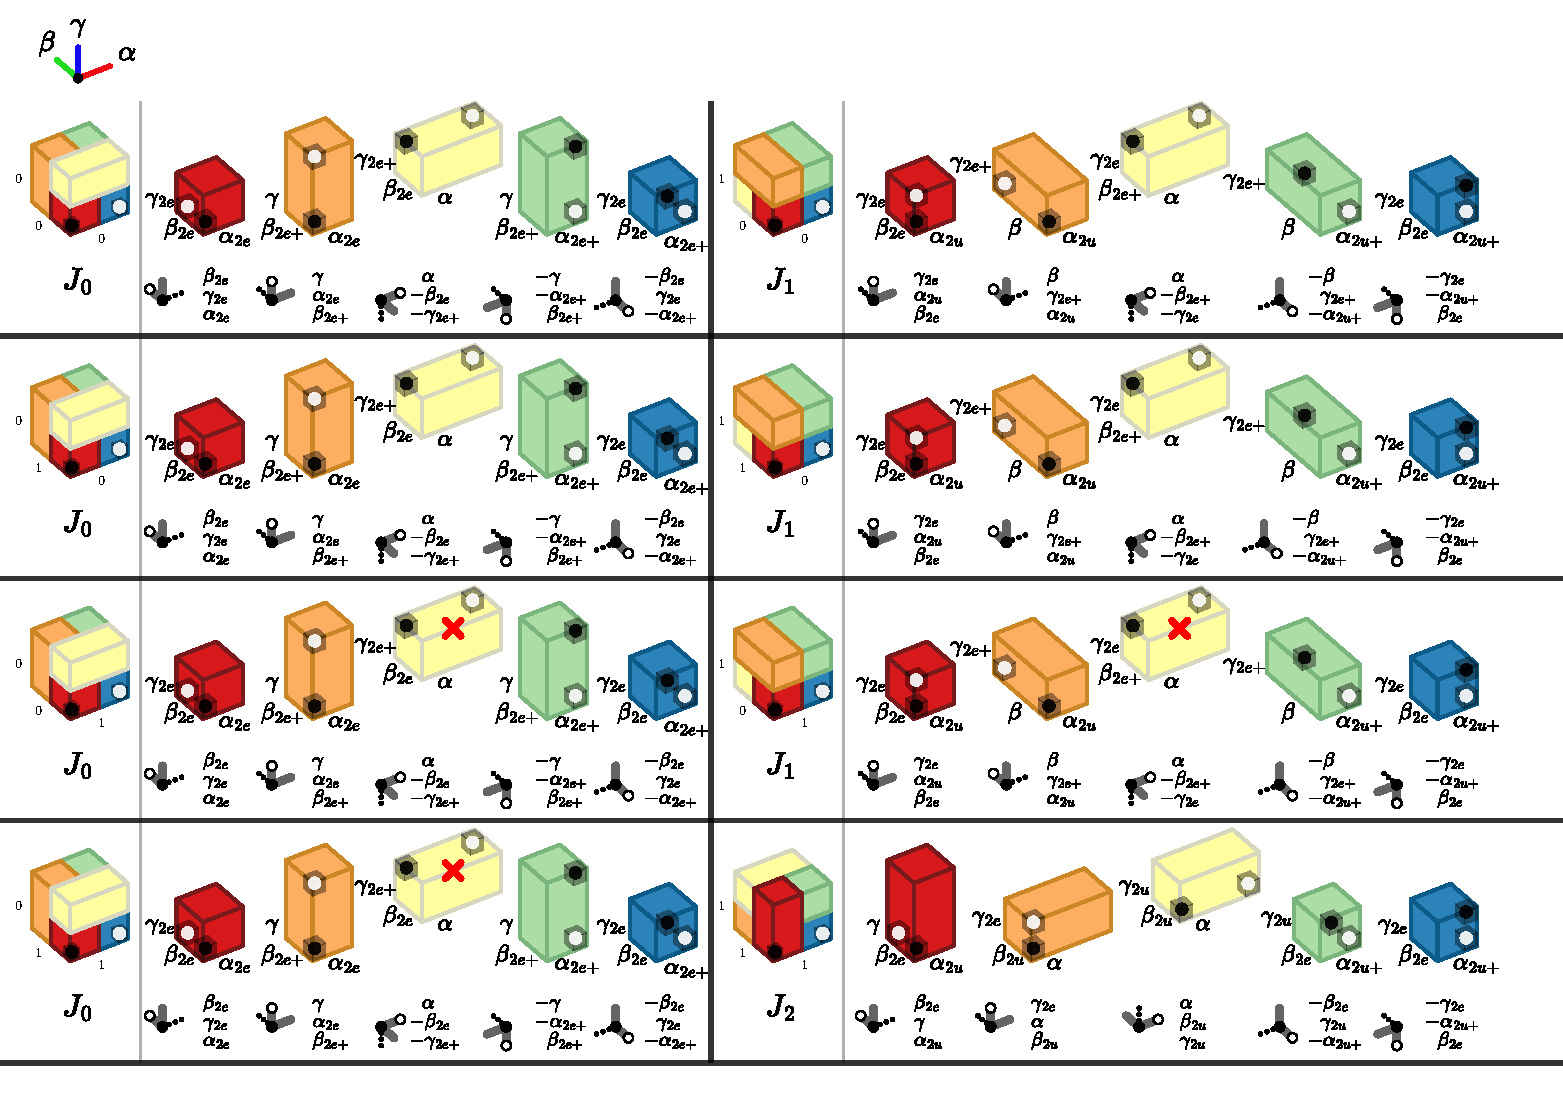
\includegraphics[width=\textwidth]{gilbert3d_case.pdf}
  \caption{ Bulk recursion J-split atlas for the 3D Gilbert algorithm }
  \label{fig:gilbert3DCase}
\end{figure*}



